\documentclass[a4paper, 10pt, final, garamond]{book}
\usepackage{cours-preambule}
\graphicspath{{./figures/}}

\makeatletter
\renewcommand{\@chapapp}{Contr\^ole de connaissances}
\makeatother

% \toggletrue{student}
% \toggletrue{corrige}
\renewcommand{\mycol}{black}
% \renewcommand{\mycol}{gray}

\begin{document}
\setcounter{chapter}{20}

\settype{enon}
\settype{solu}

\chapter{Forces centrales et chimie\ifstudent{~(13')}}

\begin{enumerate}[label=\sqenumi]
	\nitem{8}%
	Soit un point M soumis à une unique force centrale $\Ff$. Démontrer que son
	moment cinétique se conserve, justifier que son mouvement est plan et
	démontrer la loi des aires à l'aide d'un schéma. Pas besoin d'introduire la
	constante des aires.
	\smallbreak
	\begin{isd}
		\psw{
			Force centrale
			$\stm[-1]{\Lra} \Ff \parr \OM \Ra
				\Mcf_{\Or}(\Ff) \stm[-1]{=} \OM \wedge \Ff = \of$
			\begin{gather*}
				\beforetext{TMC~:}
				\boxed{\dv{\Lcf_{\Or}}{t} \stm[-1]{=} \of}
				\Lra
				\Lcf(0) = \Lc_0 \uz \stm{=} \Lcf(t)
				\\
				\beforetext{Ainsi,}
				\boxed{\OM(t) \wedge m\vf(t) \stm[-1]{=} \Lc_0 \uz} \quad \forall t
			\end{gather*}
			\smallbreak
			Pendant une durée $\dd{t}$, le point M balaye une aire $\dd{\Ac}$
			\begin{gather*}
				\dd{\Ac}            \stm{=} \frac{1}{2}\norm{\OM \wedge \vf \dd{t}}
				\Lra
				\dd{\Ac}            = \frac{1}{2}\norm{\OM \wedge m \vf} \frac{\dd{t}}{m}
				\\\Lra
				\boxed{\dv{\Ac}{t} \stm{=} \frac{\norm{\Lcf_{\Or}}}{2m} = \cte}
				\qed
			\end{gather*}
		}
		\vspace{-15pt}
		\tcblower
		\begin{center}
			\sswitch{
				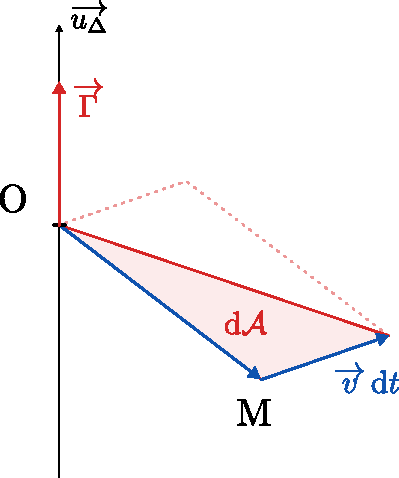
\includegraphics[scale=.6, draft=true]{dAmomcin}
			}{
				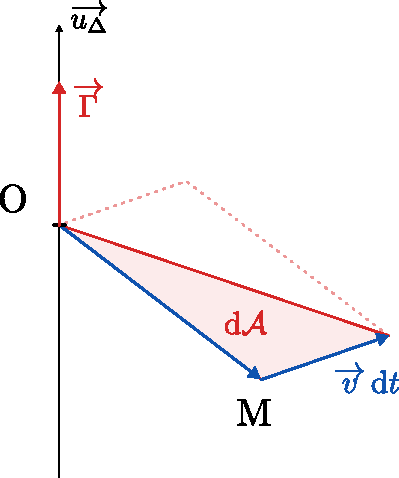
\includegraphics[scale=.6]{dAmomcin}
			}
			\captionof{figure}{Moment cinétique et aire balayée\protect\pt{1}}
		\end{center}
	\end{isd}
	% \nitem{10}%
	% Compléter le schéma du pendule pesant avec les forces et leurs moments,
	% calculés \textbf{par le bras de levier}. On suppose la liaison pivot parfaite.
	% Trouver alors l'équation du mouvement par application du \textbf{TMC scalaire
	% 	d'abord} puis \textbf{TPC ensuite}.
	% \smallbreak
	% \vspace{-15pt}
	% \noindent
	% \begin{minipage}[t]{0.70\linewidth}
	% 	\psw{
	% 		\begin{enumerate}[label=\sqenumi]
	% 			\bitem{\tikzmark{SP}Système}~: \{pendule\} solide indéformable de masse $m$
	% 			\bitem{Référentiel}~: terrestre, supposé galiléen.
	% 			\bitem{\tikzmark{RP}Repère}~:
	% 			cylindrique $(\Or,\er,\et,\ez)$ avec O centre de la liaison pivot.
	% 			\bitem{Repérage}~: $\OG = d\er$
	% 			\bitem{Bilan des actions}~:
	% 			\vspace{-15pt}
	% 			\[
	% 				\begin{array}{lcc}
	% 					\qquad\textbf{Origine}  & \textbf{Force}          & \textbf{Moment}
	% 					\\
	% 					\textbf{Poids}          & \quad \Pf = m\gf \quad~ & \Mc_z(\Pf) \stm[-1]{=}
	% 					-mgd \sin(\th)
	% 					\\
	% 					\textbf{Pivot parfaite} & \of                     & \vv{\G} \stm[-1]{=} \of
	% 				\end{array}
	% 			\]
	% 		\end{enumerate}
	% 	}
	% 	\vspace{-15pt}
	% \end{minipage}
	% \hfill
	% \begin{minipage}[t]{0.25\linewidth}
	% 	\vspace{0pt}
	% 	\begin{center}
	% 		\sswitch{
	% 			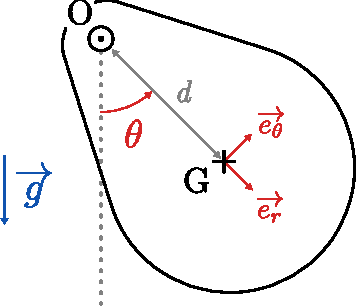
\includegraphics[width=\linewidth]{ppesant}
	% 		}{
	% 			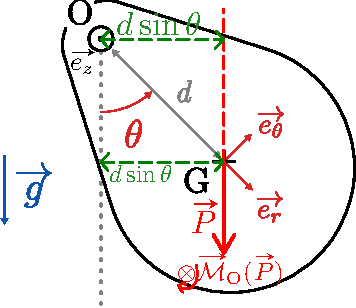
\includegraphics[width=\linewidth]{ppesant_complet}
	% 		}
	% 		\vspace{-15pt}
	% 		\captionsetup{justification=centering}
	% 		\captionof{figure}{\\Pendule pesant\protect\pt{1}}
	% 	\end{center}
	% \end{minipage}
	% \tikz[remember picture, overlay]
	% \node[below left=0pt and 20pt of pic cs:SP] {\pt{1}}
	% ;
	% \tikz[remember picture, overlay]
	% \node[below left=0pt and 20pt of pic cs:RP] {\pt{1}}
	% ;
	% \psw{
	% 	\begin{enumerate}[label=\sqenumi, start=6]
	% 		\bitem{TMC}~:
	% 		\vspace{-20pt}
	% 		\[
	% 			\dv{\Lc_z}{t} \stm{=} J_z \tpp = \Mc_z(\Pf)
	% 			\Lra
	% 			\boxed{\tpp + \frac{mgd}{J_z} \sin(\th) \stm{=} 0}
	% 		\]
	% 		\vspace{-15pt}
	% 		\bitem{TPC}~: on calcule $\Ec_c$ et $\Pc$~:
	% 		\begin{gather*}
	% 			\Ec_c = \frac{1}{2}J_z \w^2
	% 			\stm{\qet}
	% 			\Pc(\Pf) = \Mc_z(\Pf)\w
	% 			\quad \Ra \quad
	% 			\dv{\Ec_c}{t} \stm{=} \Pc(\Pf)
	% 			\Lra
	% 			J_z \dot{\w} \cancel{\w} \stm{=} -mgd\sin(\th)\cancel{\w}
	% 			\Lra
	% 			\boxed{\tpp + \frac{mgd}{J_z}\sin(\th) = 0}
	% 		\end{gather*}
	% 	\end{enumerate}
	% }
	\nitem{2}%
	Démontrer la relation de \textsc{Henderson}.
	\smallbreak
	\vspace{-30pt}
	\psw{
		\begin{DispWithArrows*}
			K_A \stm[-1](un){\triangleq}
			\frac{[\ce{H_3O+}]\ind{eq}\times [\ce{A-}]\ind{eq}}{[\ce{AH}]\ind{eq}c^\circ}
			&\Lra
			\frac{[\ce{H_3O+}]\ind{eq}}{c^\circ} =
			K_A\frac{[\ce{AH}]\ind{eq}}{[\ce{A-}]\ind{eq}}
			\CArrow{$-\log \cdot $}
			\\
			-\log [\ce{H_3O+}]\ind{eq} =
			-\log K_A - \log \frac{[\ce{AH}]\ind{eq}}{[\ce{A-}]\ind{eq}}
			& \Lra
			\boxed{\pH \stm{=} \pk + \log \frac{[\ce{A-}]}{[\ce{AH}]}}
			\qed
		\end{DispWithArrows*}
	}
	\nitem{6}%
	On mélange $V_0 = \SI{50}{mL}$ d'une solution d'acide éthanoïque de $\pk[A,1]
		= \num{4.74}$ à $c_0 = \SI{0.10}{mol.L^{-1}}$, et le même volume d'une
	solution de nitrite de sodium $\left( \ce{Na+};\ce{NO_2-} \right)$ de
	$\pk[A,2] = \num{3.2}$ à la même concentration. Déterminer l'avancement puis
	le pH.
	\smallbreak
	\noindent
	\begin{minipage}[t]{.80\linewidth}
		\begin{center}
			\def\rhgt{0.50}
			\centering
			\begin{tabularx}{\linewidth}{|l|c||YdYdYdY|}
				\hline
				\multicolumn{2}{|c||}{
					$\xmathstrut{\rhgt}$
				\textbf{Équation}\pt{1}}   &
				\psw{$\ce{CH_3COOH\aqu}$}  & $+$                    &
				\psw{$\ce{NO_2^-\aqu}$}    & $=$                    &
				\psw{$\ce{CH_3COO^-\aqu}$} & $+$                    &
				\psw{$\ce{HNO_2\aqu}$}                                \\
				\hline
				$\xmathstrut{\rhgt}$
				\tikzmark{IN}Initial       & $x = 0$                &
				\psw{$c_0/2$}              & \vline                 &
				\psw{$c_0/2$}              & \vline                 &
				\psw{$0$}                  & \vline                 &
				\psw{$0$}                                             \\
				\hline
				$\xmathstrut{\rhgt}$
				Final                      & $x_f = \psw{x_{\equ}}$ &
				\psw{$c_0/2 - x_{\equ}$}   & \vline                 &
				\psw{$c_0/2 - x_{\equ}$}   & \vline                 &
				\psw{$x_{\equ}$}           & \vline                 &
				\psw{$x_{\equ}$}                                      \\
				\hline
			\end{tabularx}
		\end{center}
		\vspace{-10pt}
		\psw{
			\begin{gather*}
				K^\circ \stm{=} \frac{x\ind{eq}^2}{\left( c_0/2-x\ind{eq} \right)^2}
				\underbracket[1pt]{\Ra}_{x\ind{eq}>0}
				x\ind{eq} = \left( \frac{c_0}{2}-x\ind{eq} \right)\sqrt{K^\circ}
				% \\\Lra
				\Lra
				\boxed{x\ind{eq} \stm{=} \frac{\sqrt{K^\circ}}{1+\sqrt{K}}\frac{c_0}{2}}
				\Ra
				\xul{x\ind{eq} = \SI{7.3e-3}{mol.L^{-1}}}\tikzmark{ANN}
				\\\Ra
				% \left\{
				% \begin{array}{rl}
				% 	[\ce{CH_3COOH}]\ind{eq}     & = [\ce{NO_2-}]\ind{eq} =
				% 	\SI{4.27e-2}{mol.L^{-1}}
				% 	\\%
				% 	\pac{\ce{CH_3COO-}}\ind{eq} & = [\ce{HNO_2}]\ind{eq} =
				% 	\SI{7.3e-3}{mol.L^{-1}}
				% \end{array}
				% \right.
				% \\\Ra
				\pH = \pk[A,1] + \log ( \frac{x\ind{eq}}{c_0/2-x\ind{eq}} ) =
				\pk[A,1] + \frac{1}{2} \log K^\circ =
				\pk[A,1] + \frac{\pk[A,2]-\pk[A,1]}{2}
				% = \pk[A,1] + \frac{1}{2} \log 10^{\pk[A,2] - \pk[A,1]}
				\Lra
				\boxed{
					\pH = \frac{\pk[A,2]+\pk[A,1]}{2} =
					\num{3.97}
				}
			\end{gather*}
		}
	\end{minipage}
	\hfill
	\begin{minipage}[t]{.15\linewidth}
		\vspace{-40pt}
		\begin{center}
			\sswitch{
				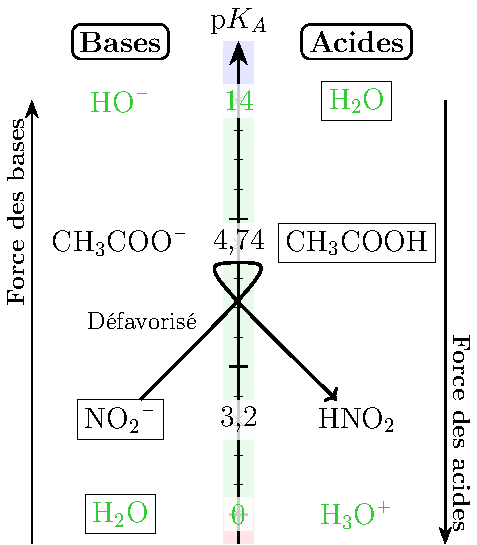
\includegraphics[width=\linewidth, draft=true]{appl_fin}
			}{
				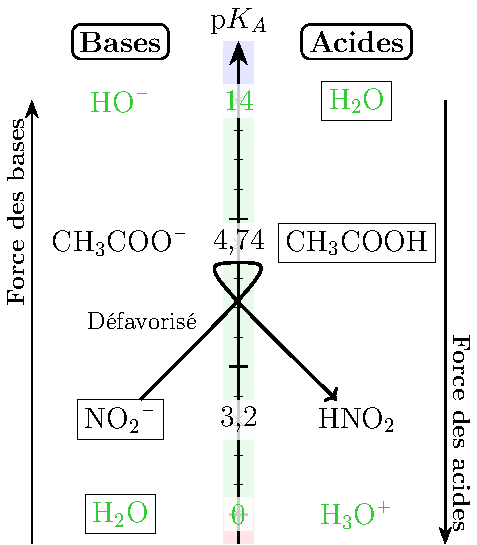
\includegraphics[width=\linewidth]{appl_fin}
			}
			% \captionof{figure}{Échelle $\pk$}
		\end{center}
	\end{minipage}
	\tikz[remember picture, overlay]
	\node[below left=0pt and 15pt of pic cs:IN] {\pt{1}}
	;
	\tikz[remember picture, overlay]
	\node at ([shift={(.5,-.25)}]pic cs:ANN) {\pt{1}}
	;
	\tikz[remember picture, overlay]
	\node at ([shift={(2.5,3)}]pic cs:ANN) {\pt{1}}
	;
	\nitem{4}%
	On ajoute $n = \SI{e-5}{mol}$ d'ions \ce{Cl-} dans $V_0 = \SI{10}{mL}$ de
	nitrate d'argent $\left( \ce{Ag+},\ce{NO_3^-} \right)$ à $c_0 =
		\SI{e-3}{mol.L^{-1}}$. On donne $\pk[s](\ce{AgCl}) = \num{9.8}$. Obtient-on un
	précipité de chlorure d'argent \ce{AgCl}~?
	\smallbreak
	\vspace{-20pt}
	\psw{
		\begin{gather*}
			\beforetext{Formation de \ce{AgCl}~:}
			\ce{Ag+\aqu{} + Cl^-\aqu{} = AgCl\sol{} \quad \pt{1}}
			\tag*{$K^\circ \stm[-1]{=} \frac{1}{K_s}$}
			\\
			\beforetext{Sens direct $\Ra$}
			Q_{r,i} < \frac{1}{K_s}
			\Lra
			\frac{{c^\circ}^2}{[\ce{Ag+}]_i[\ce{Cl-}]_i} < \frac{1}{K_s}
			\Lra
			\boxed{\frac{[\ce{Ag+}]_i[\ce{Cl-}]_i}{{c^\circ}^2} \stm{>} K_s}
			\\\AN
			[\ce{Ag+}]_i = \SI{e-3}{mol.L^{-1}}
			\qet
			[\ce{Cl-}]_i = n/V_0 = \SI{e-3}{mol.L^{-1}}
			\quad \Ra \quad
			\xul{\frac{[\ce{Ag+}]_i[\ce{Cl-}]_i}{{c^\circ}^2} \stm{=} \num{e-6} > K_s}
		\end{gather*}
	}
	\vspace*{-15pt}
	\ifstudent{
		\begin{tikzpicture}[remember picture, overlay]
			\node[anchor=north west, align=left]
			at ([shift={(1.4cm,0)}]current page.north west)
			{\\[5pt]\Large\bfseries Nom~:\\[10pt]\Large\bfseries Prénom~:};
			\node[anchor=north east, align=right]
			at ([shift={(-1.5cm,-17pt)}]current page.north east)
			{\Large\bfseries Note~:\hspace{1cm}/20};
		\end{tikzpicture}
	}
\end{enumerate}
\end{document}
